
\documentclass{article}
\usepackage[final]{neurips_2023}
\usepackage[utf8]{inputenc}
\usepackage[T1]{fontenc}
\usepackage{hyperref}
\usepackage{url}
\usepackage{booktabs}
\usepackage{amsfonts,amsmath}
\usepackage{microtype}
\usepackage{graphicx}
\graphicspath{{figures/}}
\usepackage{xcolor}
\setlength{\textfloatsep}{5pt plus 2pt minus 2pt}
\setlength{\floatsep}{6pt plus 2pt minus 2pt}
\setlength{\abovecaptionskip}{3pt}
\setlength{\belowcaptionskip}{0pt}
\renewcommand{\topfraction}{0.9}\renewcommand{\bottomfraction}{0.9}\renewcommand{\textfraction}{0.05}
\renewcommand{\floatpagefraction}{0.8}
\title{Spectrally Normalized Residual GAN for WikiArt Painting Synthesis}
\author{Meng-Chi Tsai \\ PID: A69042039 \\ ECE 285, Homework 2 \quad \href{https://github.com/moose1108/ece285-homeworks/tree/main/HW2}{Code and results (GitHub)}}
\begin{document}
\maketitle
\begin{abstract}
We train a spectrally normalized residual GAN (hinge loss, two time-scale updates, EMA generator) on
73{,}313 WikiArt paintings at $64\times64$ resolution. Evaluated against 8{,}131 held-out paintings with
PyTorch-Ignite, the EMA generator obtains FID 25.05 and Inception Score 5.13
(real held-out images: IS 7.49; train-vs-held-out FID floor 7.19).
\end{abstract}

\section{Data and model}
\textbf{Data.} We use all 81{,}444 WikiArt images (27 styles), resized (bicubic) so the short side is 64\,px and
center-cropped. A filename-hash split gives 73{,}313 training and 8{,}131 held-out images; training adds random horizontal flips.

\textbf{Architecture.} The generator maps $z\sim\mathcal N(0,I_{128})$ to a $4{\times}4$ map with a linear layer, then applies four residual
up-sampling blocks (BN--ReLU--upsample--conv$3{\times}3$; widths 384/384/192/96/48) and a BN--ReLU--conv--tanh head (5.0M parameters).
The discriminator has five residual blocks with spectral normalization~[1] on every layer, global sum pooling and a linear head (5.5M parameters).

\textbf{Objective and training.} We minimize the hinge loss~[2],
$\mathcal L_D=\mathbb E_x[\max(0,1-D(x))]+\mathbb E_z[\max(0,1+D(G(z)))]$ and $\mathcal L_G=-\mathbb E_z[D(G(z))]$,
with one update of each network per step, Adam$(0,0.9)$, and a 4$\times$ larger learning rate for $D$ than for $G$~[3]
(held for the first half of training, then decayed linearly; fp16 mixed precision).
Reported images and metrics use an exponential moving average of the generator~[4,5] with warm-up
(decay $\min(0.999,\frac{1+t}{10+t})$) whose BatchNorm statistics are re-estimated from 25k samples instead of being copied.

\begin{table}[!htb]
\centering\small
\caption{Hyperparameters of the final run.}
\begin{tabular}{ll@{\qquad}ll}
\toprule
Resolution & $64\times64$ & Batch size & 64 \\
Latent dimension & 128 & Epochs / iterations & 52 / 59{,}540 \\
Learning rate $D$ / $G$ & $4{\times}10^{-4}$ / $1{\times}10^{-4}$ & Adam $(\beta_1,\beta_2)$ & $(0,\,0.9)$ \\
Loss & hinge & EMA decay & 0.999 (warm-up) \\
Base width & 48 & Random seed & 285 \\
\bottomrule
\end{tabular}
\end{table}

\begin{figure}[!b]
\centering
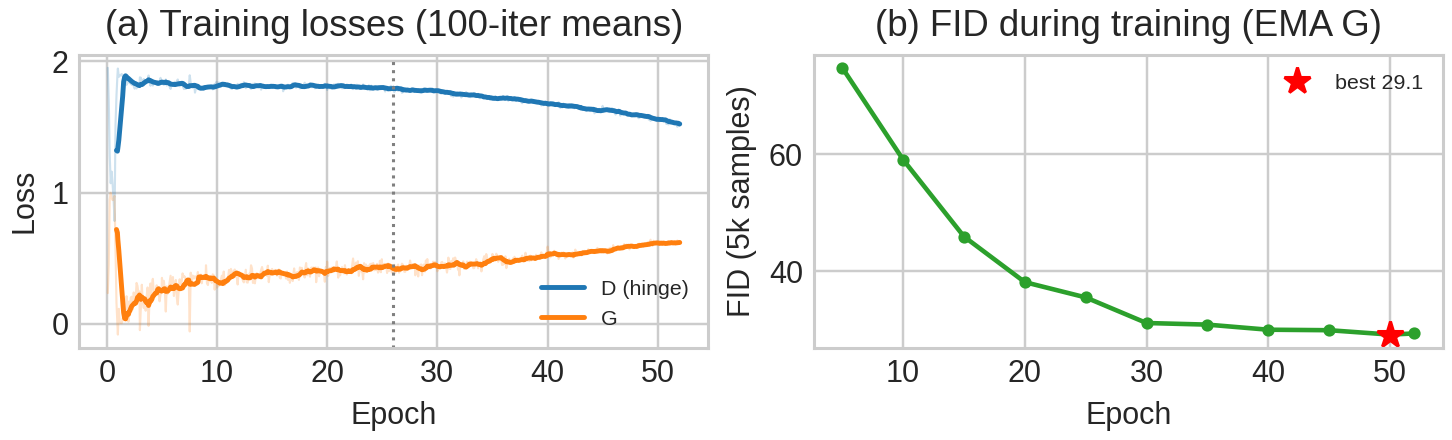
\includegraphics[width=0.500\linewidth]{fig_training.png}
\caption{(a) Generator and discriminator losses (dotted line: start of learning-rate decay). (b) FID of the EMA generator during training.}
\label{fig:train}
\end{figure}

\section{Evaluation protocol}
Both metrics use the PyTorch-Ignite implementations from the assignment. Images are resized bilinearly to $299{\times}299$, ImageNet-normalized and passed
through Inception-v3; generated images are first quantized to 8 bits. FID~[3] uses the 2048-d pool features and IS~[6] the softmax output, computed on
8{,}131 generated images versus the 8{,}131 held-out real images. Ignite's \texttt{FID()} defaults to the 1000-d \emph{softmax} output, whose scale is
not comparable with published FIDs (FID$^\dagger$ in Table~\ref{tab:res}), so we specify the 2048-d features explicitly. As references (Table~\ref{tab:res}) we use real training images vs.\ held-out images (FID) and the IS of real held-out images.

\section{Results}
See Fig.~\ref{fig:train} (training), Table~\ref{tab:res} (metrics) and Fig.~\ref{fig:samples} (samples).
The monitor FID falls from 74.8 (epoch 5) to 29.1 (epoch 50). Over the last epochs the discriminator loss is 1.52 (chance level is 2) with mean scores
$D(x)=+0.05$ and $D(G(z))=-0.61$, so neither network overpowers the other. Samples reproduce the global palette, brush-stroke texture and composition statistics of the collection, whereas fine object structure (faces, buildings) is rarely coherent; this is typical of unconditional GANs on a stylistically very diverse dataset at $64{\times}64$ resolution. Because FID and IS rely on ImageNet features that only loosely capture artistic style, we read them together with the samples.

\begin{table}[!htb]
\centering\small
\caption{Results on 8{,}131 held-out images (lower FID, higher IS is better). FID$^\dagger$: Ignite default (softmax features).}
\label{tab:res}
\begin{tabular}{lccc}
\toprule
Model & FID $\downarrow$ & IS $\uparrow$ & FID$^\dagger$ \\
\midrule
SN-ResNet GAN + EMA (ours, epoch 50) & 25.05 & 5.13 & 0.0354 \\
Real train subset vs.\ held-out (reference) & 7.19 & 7.49 & -- \\
\bottomrule
\end{tabular}
\end{table}

\begin{figure}[!htb]
\centering
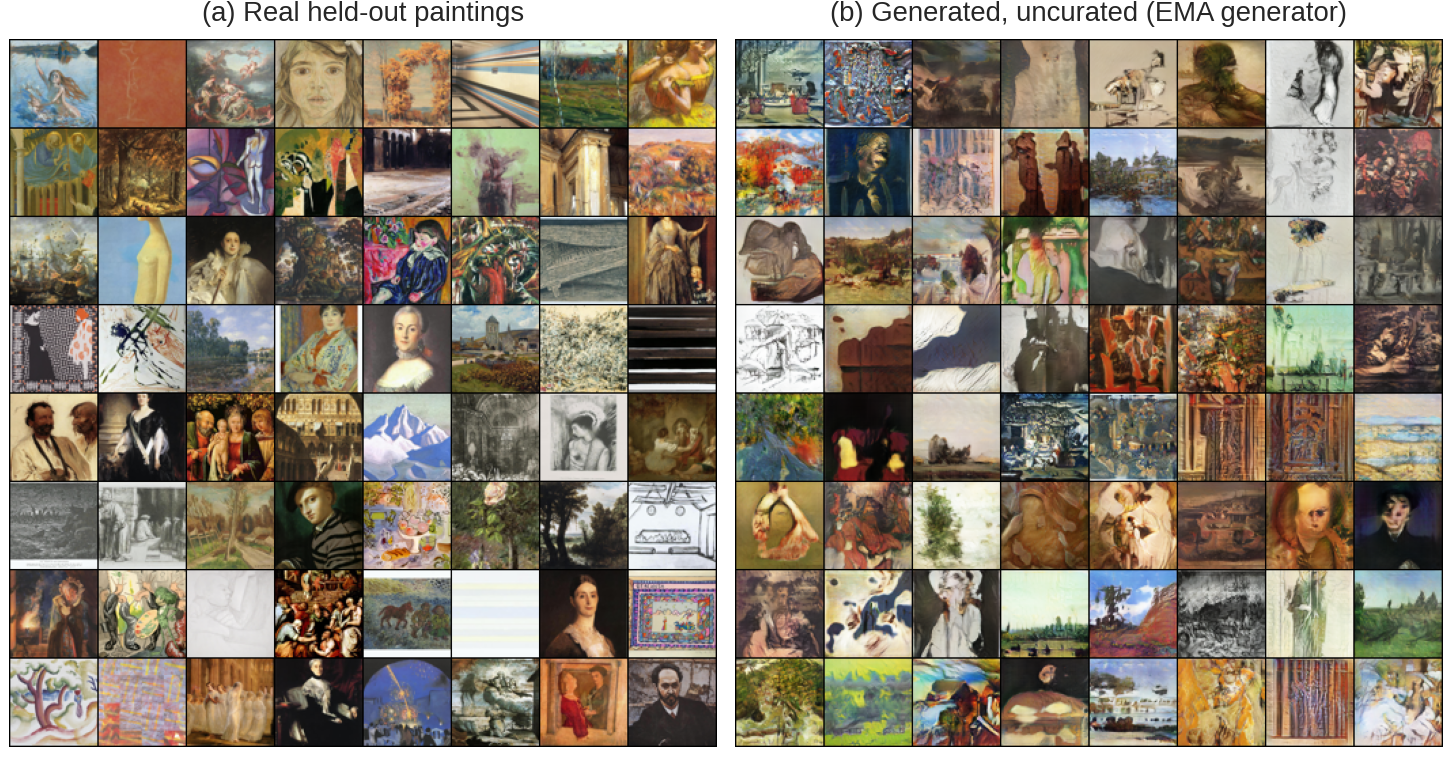
\includegraphics[width=0.650\linewidth]{fig_samples.png}
\caption{Uncurated samples of the EMA generator (right) next to random held-out paintings (left).}
\label{fig:samples}
\end{figure}

\section{Discussion}
\textbf{What mattered.} Our first attempt (a plain DCGAN trained for 8 epochs, about 2.3k iterations) collapsed to near-uniform olive images (IS 1.10).
Three changes fixed this: (i) caching the dataset as $64{\times}64$ uint8 tensors on the GPU removed the JPEG-decoding bottleneck (an epoch now takes 176\,s),
allowing 59{,}540 iterations instead of 2.3k; (ii) a bias-corrected EMA generator with re-estimated BatchNorm statistics (the naive EMA still contained
about 10\% of the random initialization); (iii) a residual spectrally normalized discriminator trained with a 4$\times$ higher learning rate than the generator, since the
first discriminator's hinge loss stayed near its chance level of 2. Remaining limitations are the low $64{\times}64$ resolution, the lack of
style conditioning, and center-cropping, which discards the borders of non-square paintings.

\noindent\textbf{References.}
{\scriptsize
[1] T.~Miyato et al. Spectral normalization for GANs. ICLR 2018.\quad
[2] J.~H.~Lim, J.~C.~Ye. Geometric GAN. arXiv:1705.02894.\quad
[3] M.~Heusel et al. GANs trained by a two time-scale update rule (introduces FID). NeurIPS 2017.\quad
[4] Y.~Yazici et al. The unusual effectiveness of averaging in GAN training. ICLR 2019.\quad
[5] A.~Brock et al. Large scale GAN training for high fidelity natural image synthesis. ICLR 2019.\quad
[6] T.~Salimans et al. Improved techniques for training GANs (introduces IS). NeurIPS 2016.\par}
\end{document}
